
This chapter presents the results obtained during the development and testing of the modular charging station and the instrumented drone. The results include the functionality tests of the charging station, flight tests, ArUco marker detection, and communication between the various components.

\section{Final Design of the First Prototype of the Charging Station}

The final design of the charging station prototype was successfully constructed and tested. Figures \ref{fig:charging_station_assembled_1} and \ref{fig:charging_station_assembled_2} show the assembled modular charging station, including the internal and external drawers, telescopic rails, and the mechanism for drawer movement.

\begin{figure}[H]
    \centering
    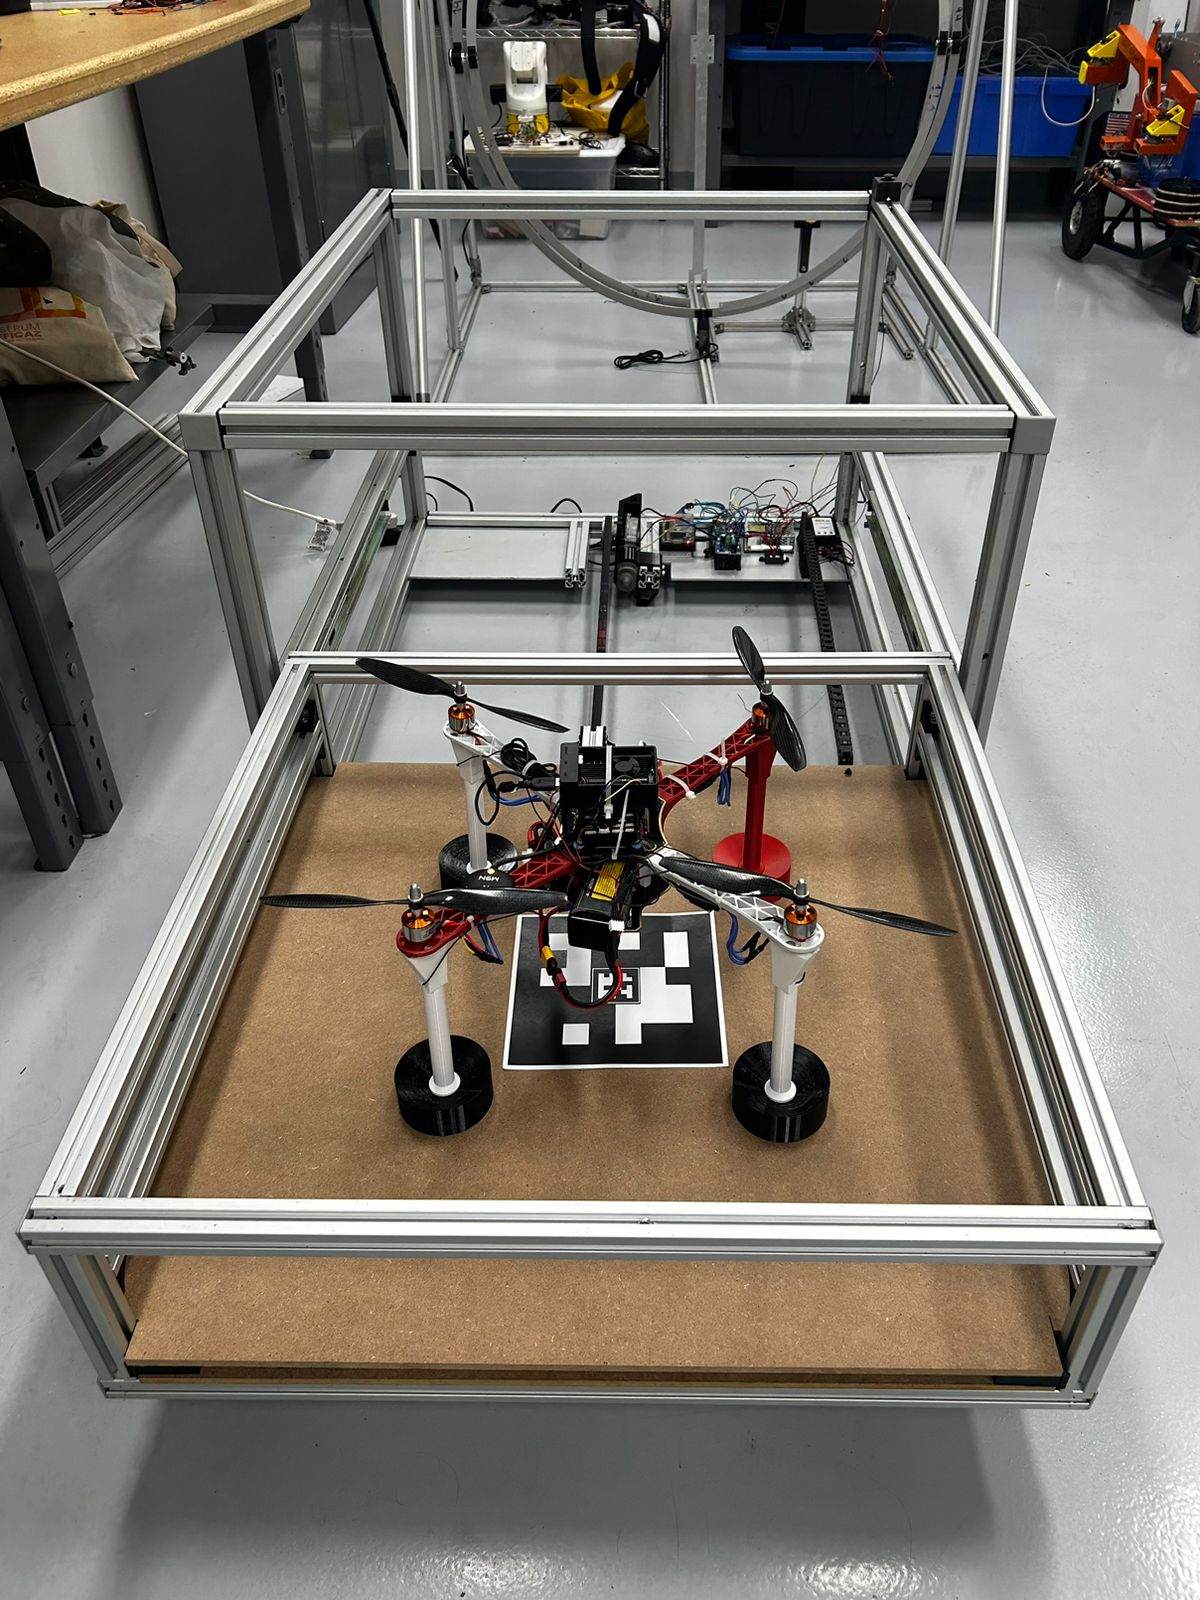
\includegraphics[width=0.4\textwidth]{pictures/ESTACION_FINAL.jpg}
    \caption{Front view of the final prototype of the modular charging station.}
    \label{fig:charging_station_assembled_1}
\end{figure}

\begin{figure}[H]
    \centering
    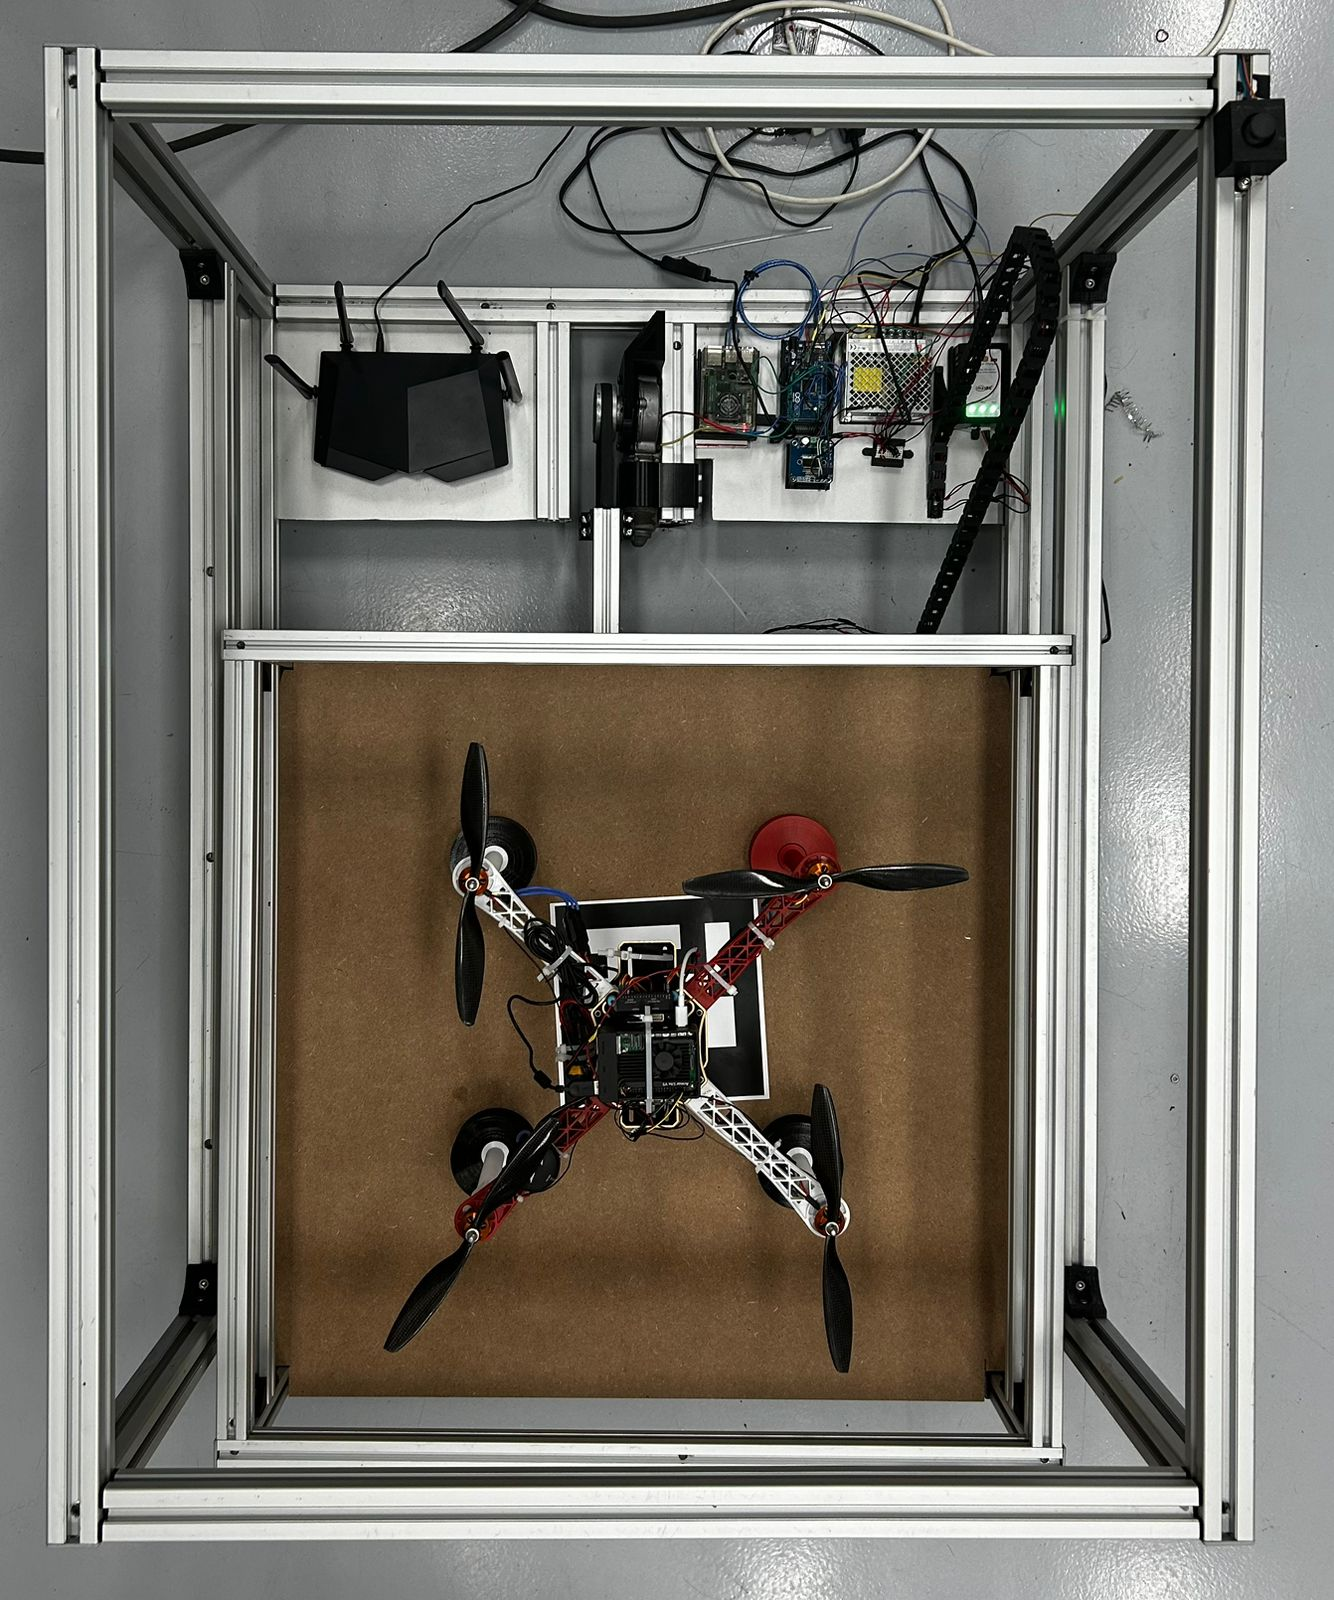
\includegraphics[width=0.4\textwidth]{pictures/charg_station_top.jpeg}
    \caption{Top view of the final prototype of the modular charging station, showing the internal drawer.}
    \label{fig:charging_station_assembled_2}
\end{figure}

\section{Design and Instrumentation of the Drone}

The drone was equipped with the necessary components to ensure seamless integration with the charging station. The mounting of the Raspberry Pi, camera, GPS module, and other sensors is illustrated in Figures \ref{fig:drone_instrumentation_1} and \ref{fig:drone_instrumentation_2}.

\begin{figure}[H]
    \centering
    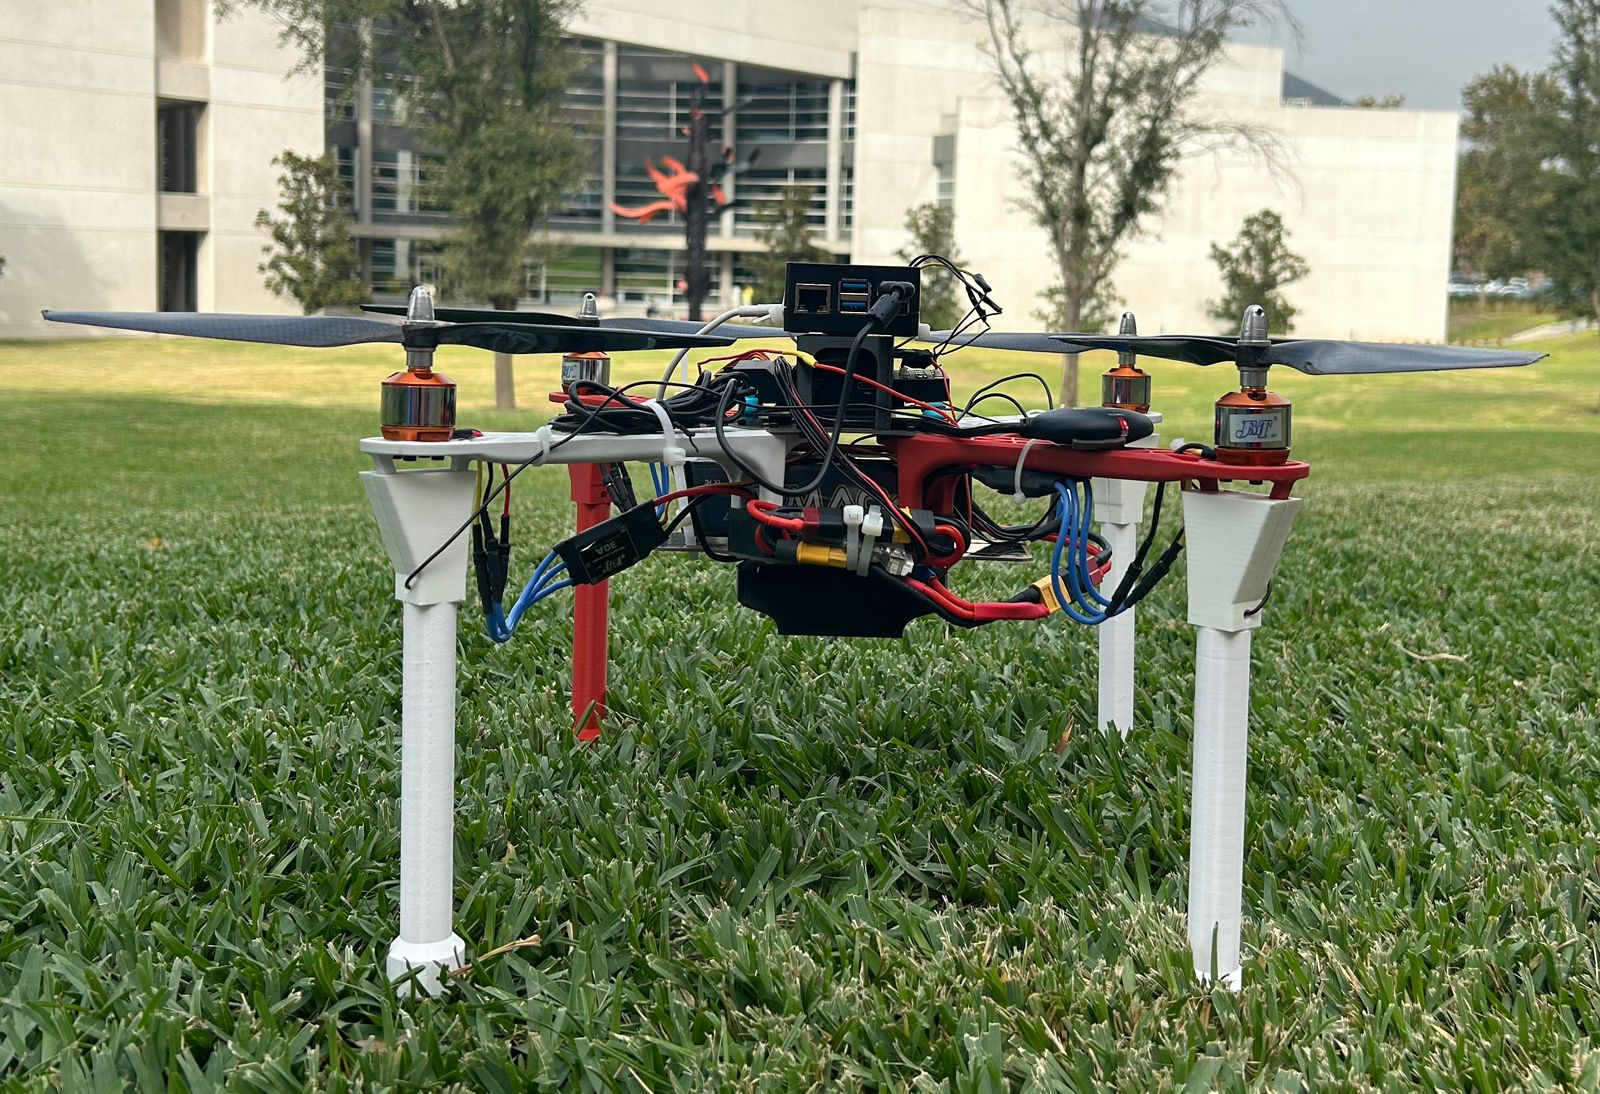
\includegraphics[width=0.4\textwidth]{pictures/drone_side_view.jpeg}
    \caption{Side view of the instrumented drone, showing the Raspberry Pi and camera integration.}
    \label{fig:drone_instrumentation_1}
\end{figure}

\begin{figure}[H]
    \centering
    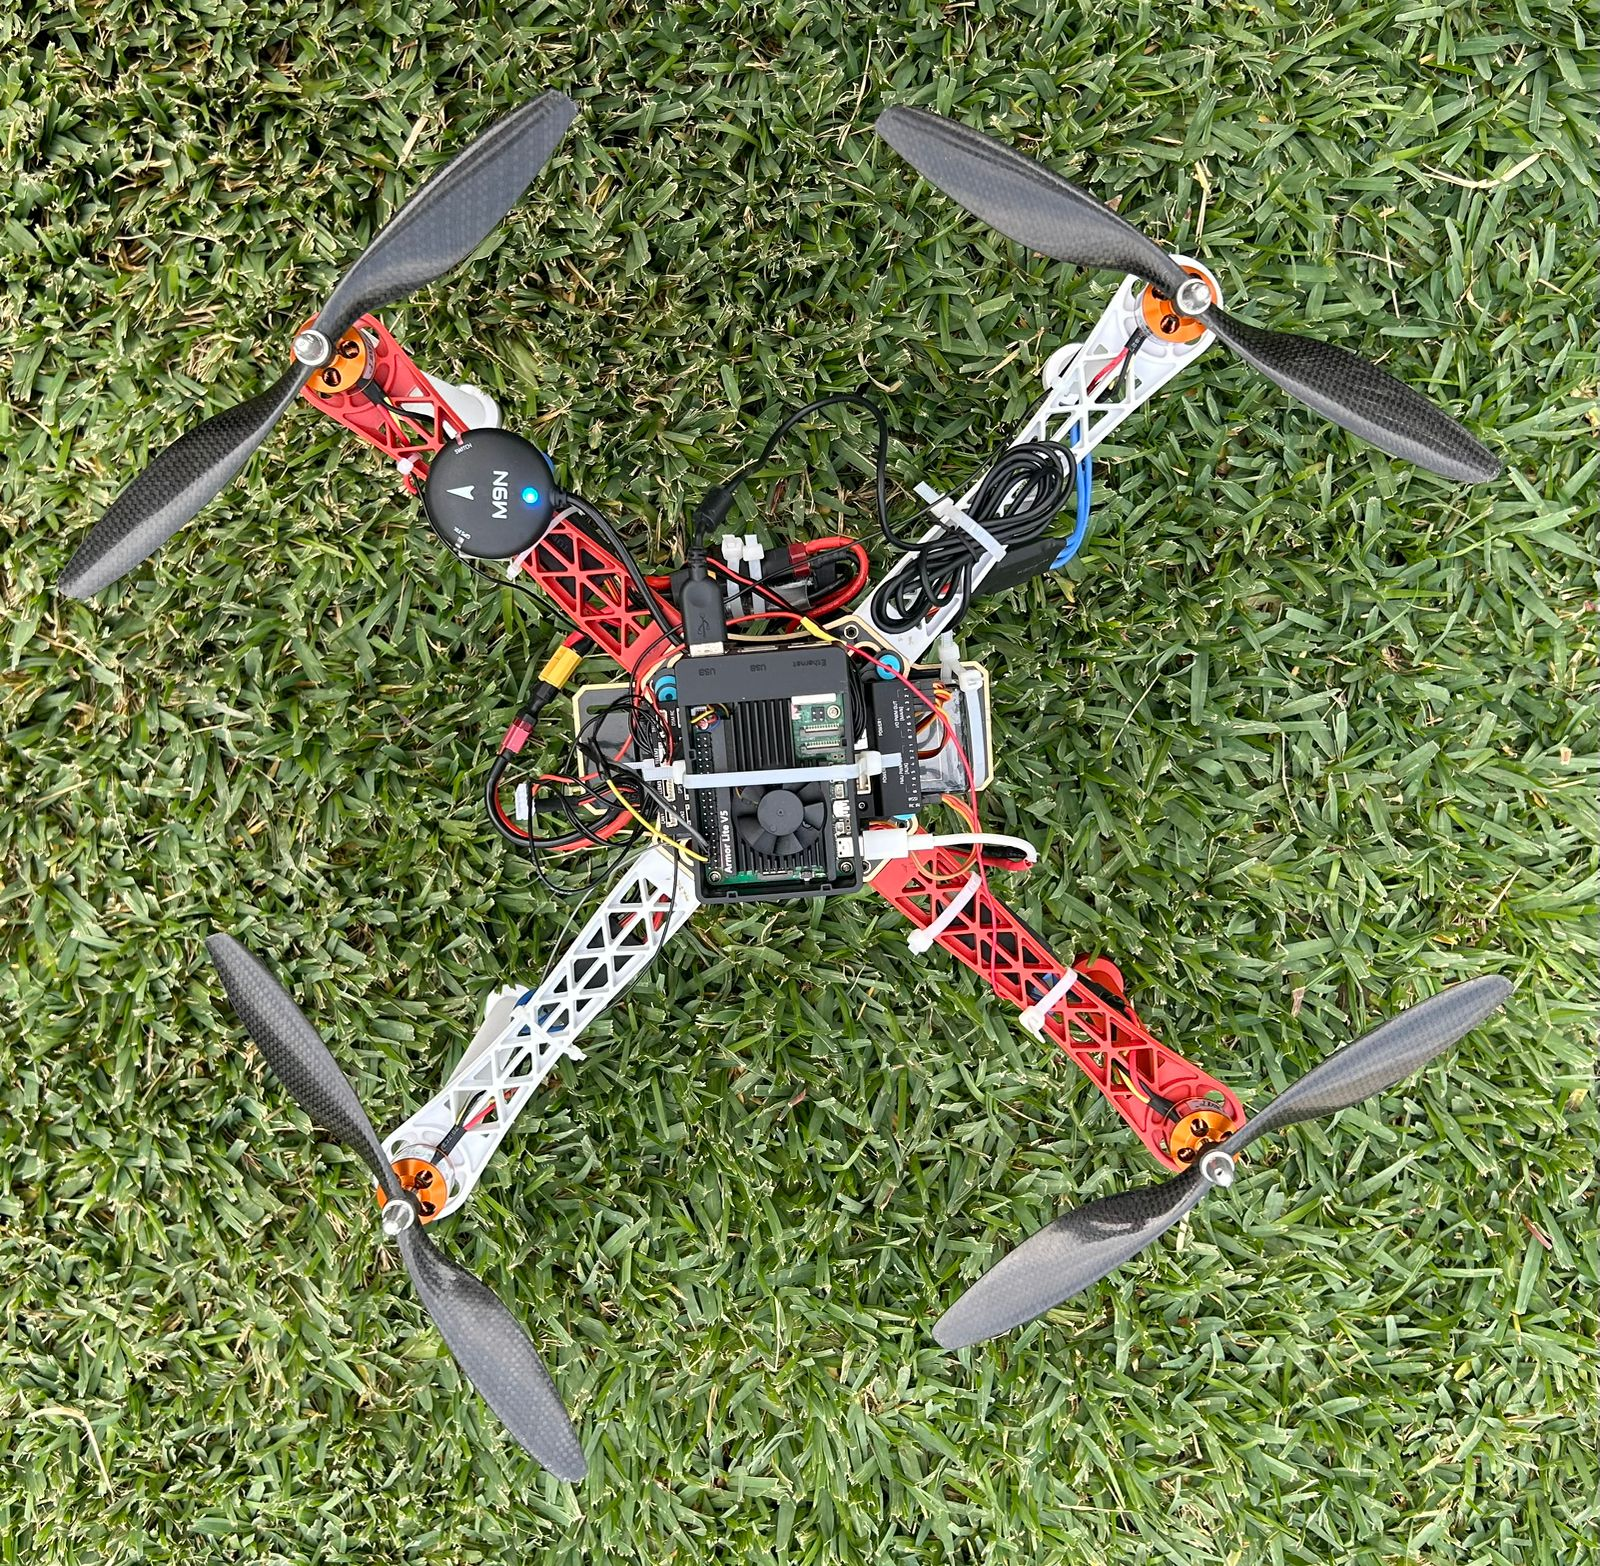
\includegraphics[width=0.4\textwidth]{pictures/drone_top_view.jpeg}
    \caption{Top view of the instrumented drone with the GPS module and charging connectors.}
    \label{fig:drone_instrumentation_2}
\end{figure}

\section{Drawer Movement}

The drawer's movement mechanism was tested under various conditions to ensure smooth and reliable operation. The motor-driven V-belt and pulley system successfully opened and closed the drawer without obstructions. Figure \ref{fig:drawer_movement} shows the drawer in motion.

\begin{figure}[H]
    \centering
    \begin{subfigure}[H]{0.45\textwidth}
        \centering
        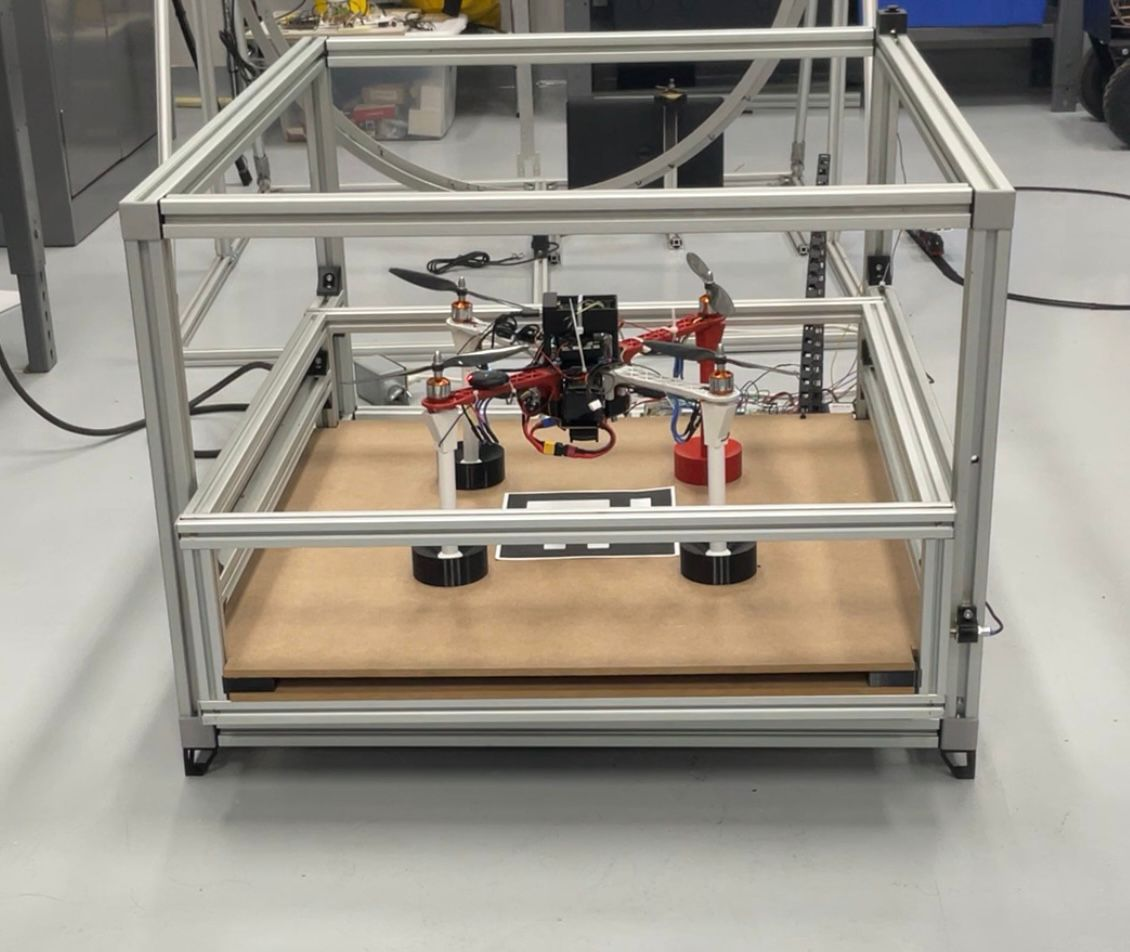
\includegraphics[width=0.8\textwidth]{pictures/drawer_open.jpeg}
        \label{fig:drawer_open}
    \end{subfigure}
    \begin{subfigure}[H]{0.45\textwidth}
        \centering
        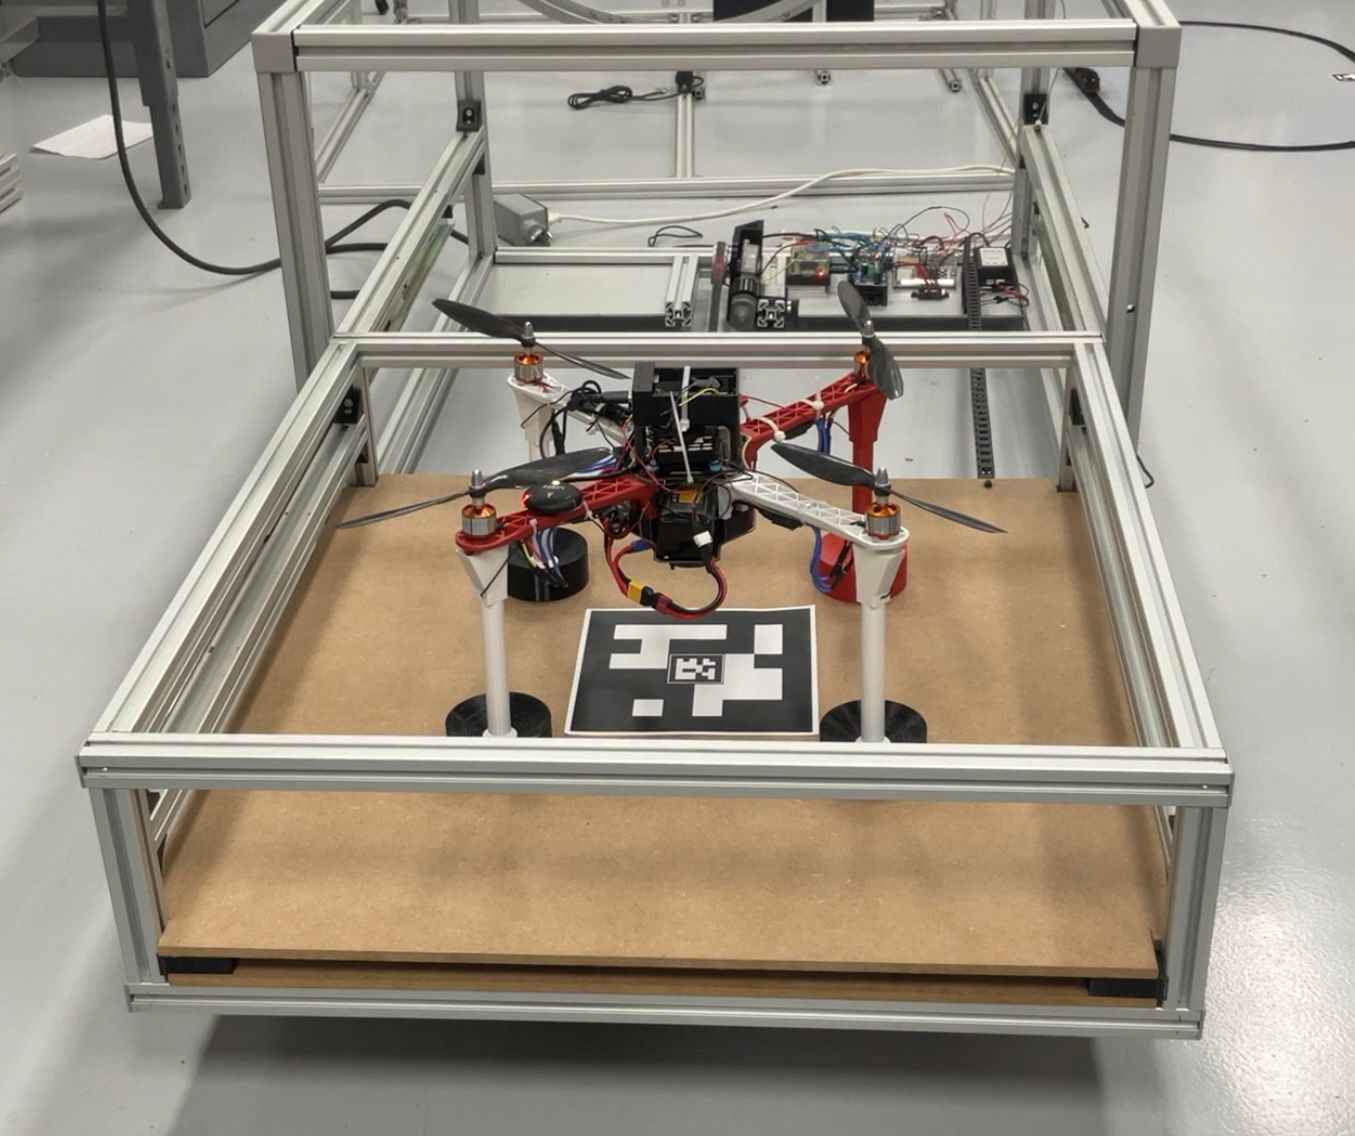
\includegraphics[width=0.8\textwidth]{pictures/drawer_closed.jpeg}
        \label{fig:drawer_closed}
    \end{subfigure}
    \caption{Movement of the drawer during opening and closing operations.}
    \label{fig:drawer_movement}
\end{figure}

\section{Drone Flight}

The drone underwent flight tests to evaluate its stability and functionality. The tests demonstrated that the drone could maintain a steady hover and fly manually with stability. Additionally, position control commands were successfully executed in outdoor environments, leveraging the GPS module for accurate positioning.

However, due to the lack of indoor positioning sensors, it was not possible to conduct position-controlled flight tests indoors. Figure \ref{fig:drone_flight_test} illustrates the drone during one of the test flights.

\begin{figure}[H]
    \centering
    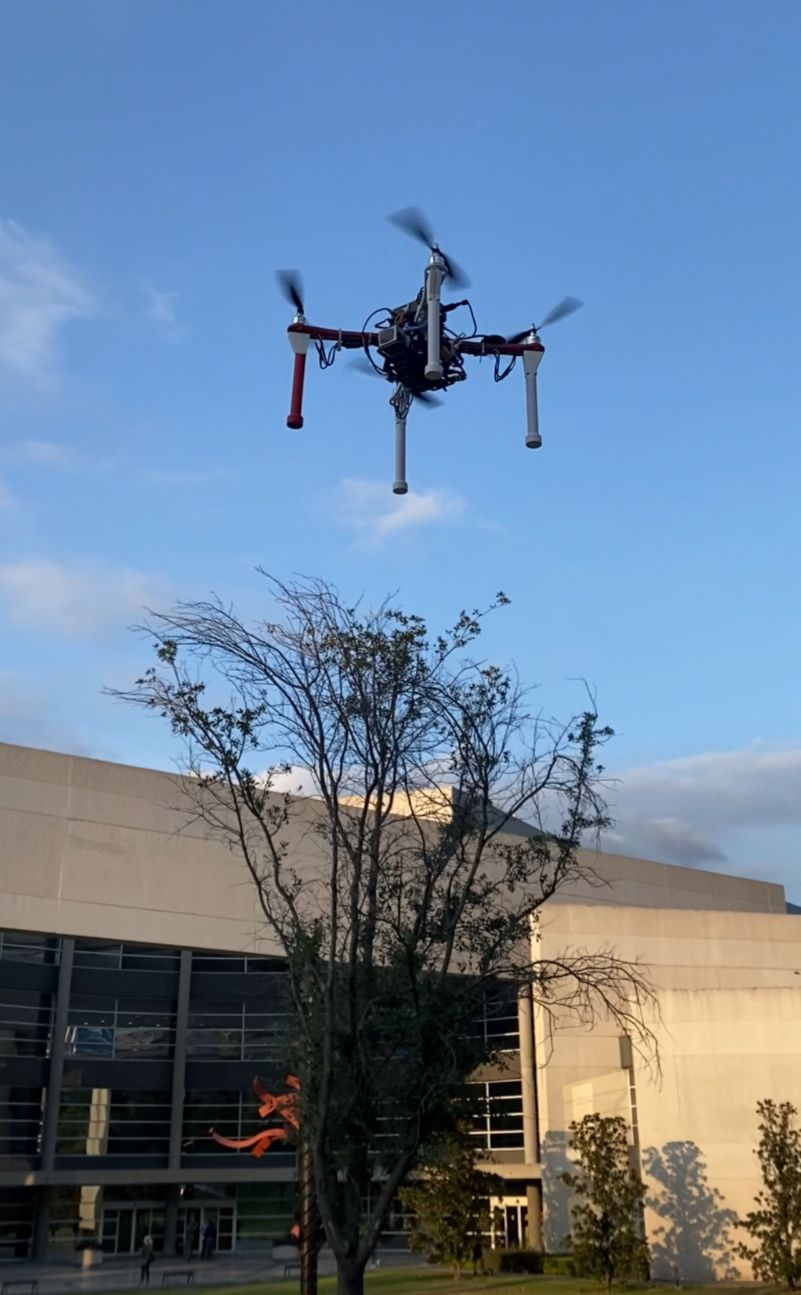
\includegraphics[width=0.4\textwidth]{pictures/drone_volando.jpeg}
    \caption{The drone in flight, performing stability and navigation tests.}
    \label{fig:drone_flight_test}
\end{figure}

\section{Battery Charging and Discharging}

Battery charging and discharging tests were conducted to measure the station's efficiency and ensure proper functioning. The tests considered two scenarios: when the drone is outside the charging station and when it is inside the station but not flying. In all tests, the motors remained inactive to isolate the power consumption of the Pixhawk and Raspberry Pi.

\subsection{Battery Duration Without Charging}

When the drone operates outside the charging station and without motor activity, the battery discharges at a faster rate due to the constant consumption by the Pixhawk and Raspberry Pi. Under these conditions, the battery lasts approximately 110 minutes before reaching the critical voltage of 9.8 V, at which point the system shuts down completely. Figure \ref{fig:battery_charging_curve} illustrates the discharge curve for this scenario.

\begin{figure}[H] 
    \centering 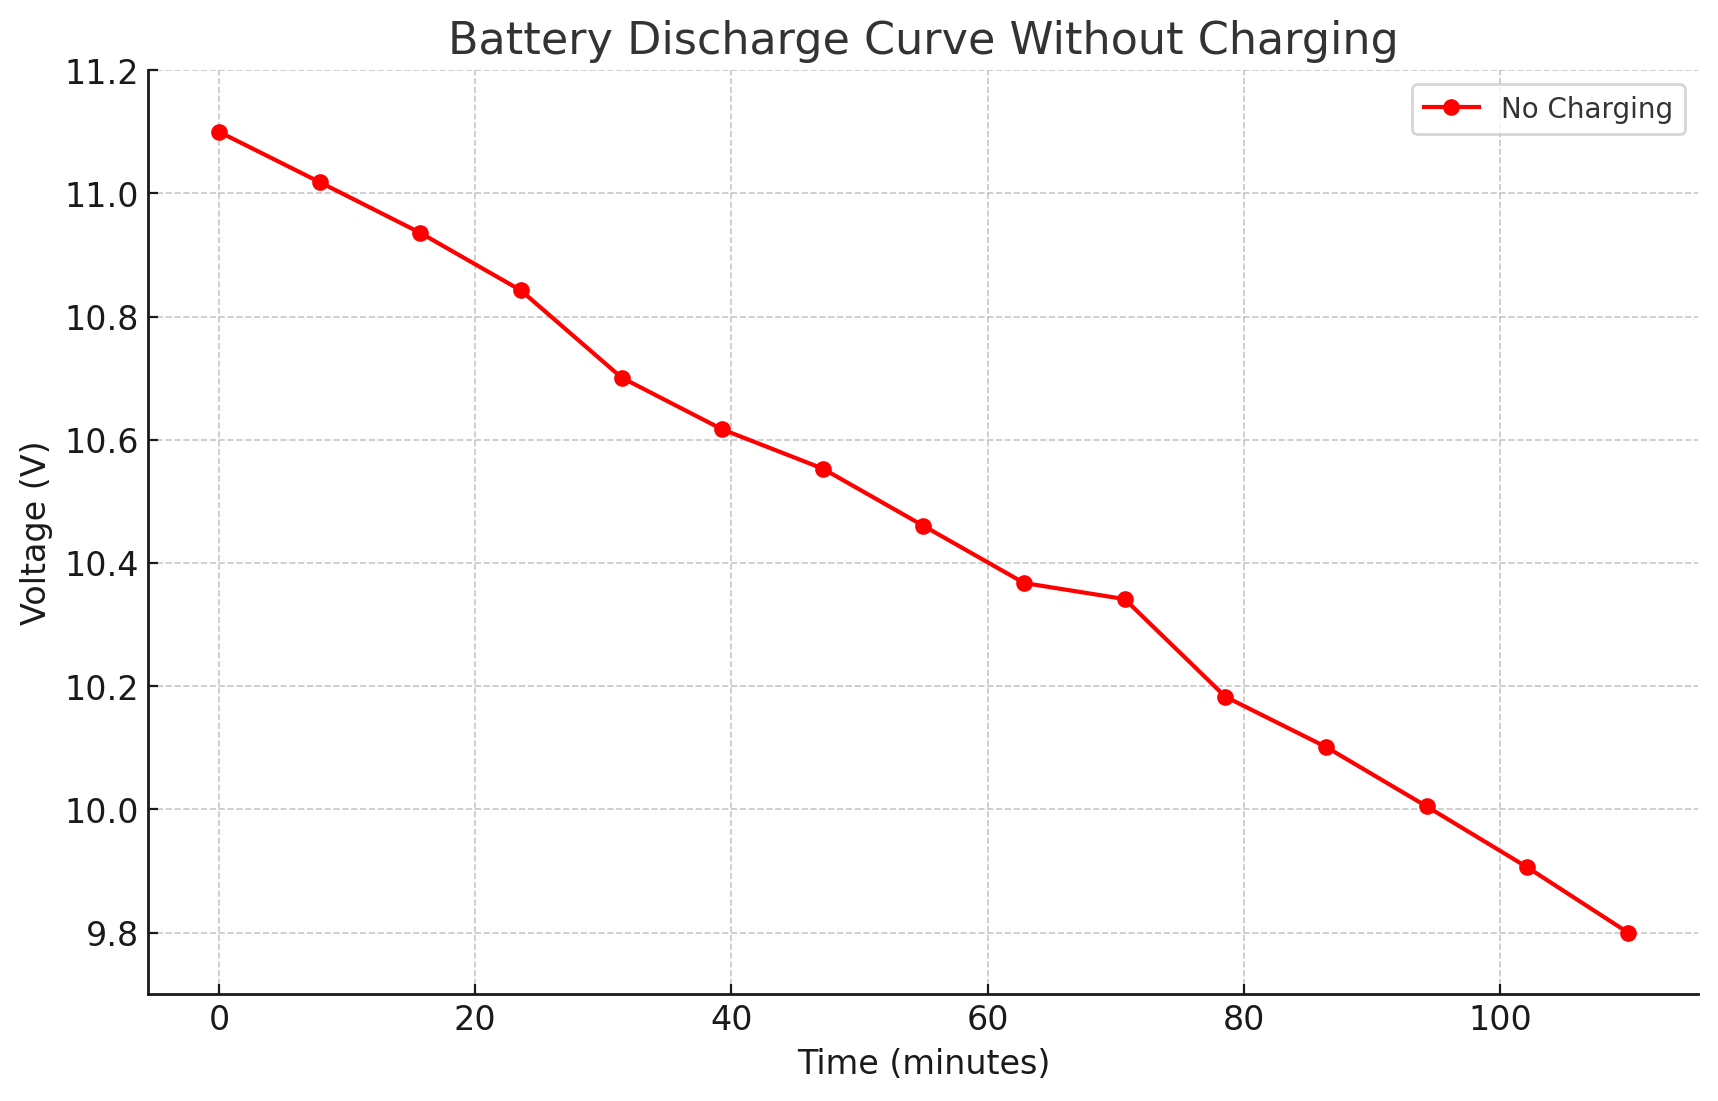
\includegraphics[width=0.8\textwidth]{pictures/Battery_Discharge_Outside.png} 
    \caption{Battery discharging curve outside the charging station, showing voltage over time.} 
    \label{fig:battery_charging_curve} 
\end{figure}

Figure 4.8 demonstrates the battery discharging curve while connected to the station. The graph shows that even with the connection to a small charger, the battery continues to discharge, though at a slower rate. This indicates that the charger's capacity is insufficient to fully counterbalance the power consumption, merely reducing the discharge rate rather than preventing it entirely.

\subsection{Battery Duration While Inside the Charging Station}

While inside the charging station, the small charger provides some support to the battery, significantly slowing the discharge rate. However, due to the charger’s limited capacity, the battery continues to discharge slowly instead of gaining charge. Under these conditions, the battery lasts approximately 190 minutes before reaching the critical voltage of 9.8 V. Figure \ref{fig:battery_discharge_curve} illustrates the discharge curve for this scenario.

\begin{figure}[H]
    \centering
    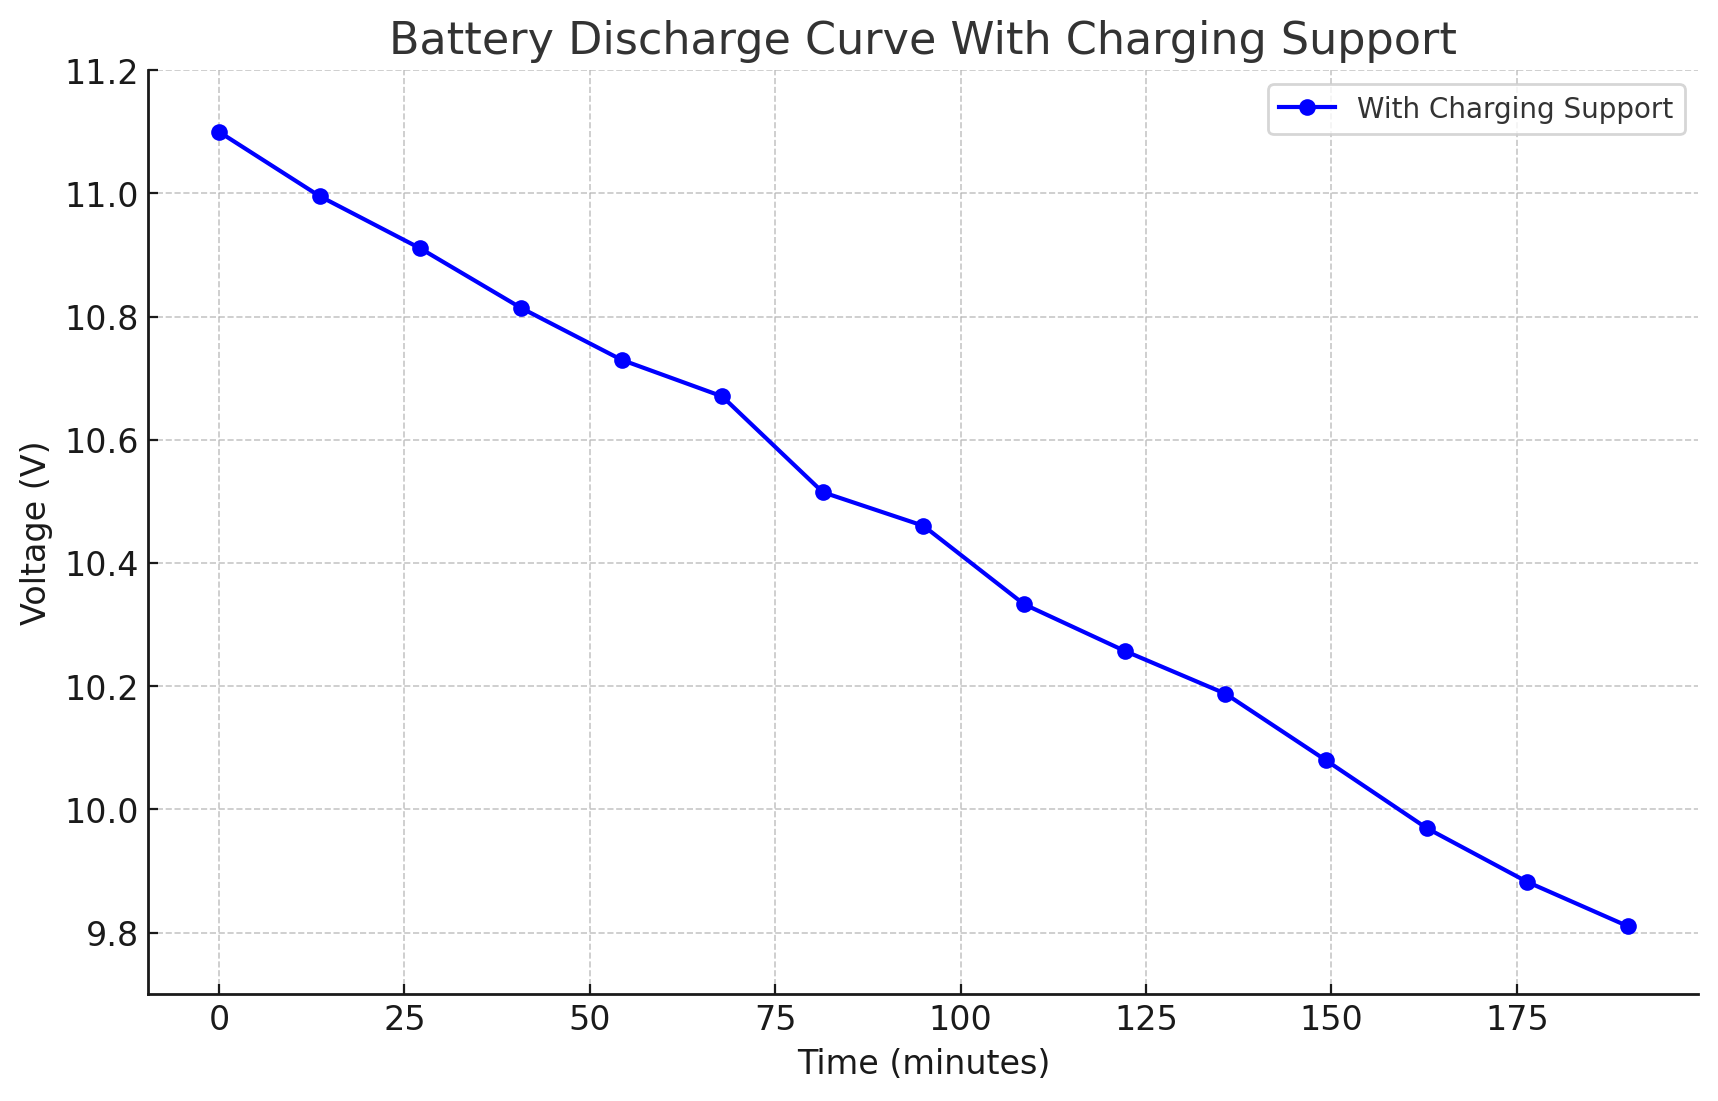
\includegraphics[width=0.8\textwidth]{pictures/Battery_Discharge_Inside.png}
    \caption{Battery discharging curve while connected to the station. The small charger only slows the discharge rate.}
    \label{fig:battery_discharge_curve}
\end{figure}

\subsection{Flight Duration}

While the drone is flying, the motors significantly increase the power consumption, reducing the battery duration to approximately 20 minutes. This demonstrates the high demand placed on the battery during active flight, which is much shorter compared to stationary operations.

\subsection{Recommendations for Improvement}

To enhance the charging system:
\begin{itemize}
    \item Replace the current charger with a higher-capacity model that can fully charge the battery while powering the Pixhawk and Raspberry Pi.
    \item Implement a power management system that disconnects non-critical components during charging cycles to prioritize battery recovery.
\end{itemize}


\section{ArUco Marker Detection}

The vision system successfully detected ArUco markers in real-time, providing accurate position and orientation data for the drone. Using the camera mounted on the drone and the OpenCV ArUco library, the system calculated the following parameters relative to the detected markers:
\begin{itemize}
    \item \textbf{Position (X, Y, Z):} The system determined the translation vector (\texttt{tvec}) representing the drone's position in meters relative to the marker.
    
    \item \textbf{Orientation (Pitch, Roll, Yaw):} The rotation vector (\texttt{rvec}) was converted into Euler angles to represent the drone's orientation in 3D space.
    
    \begin{figure}[H]
        \centering
        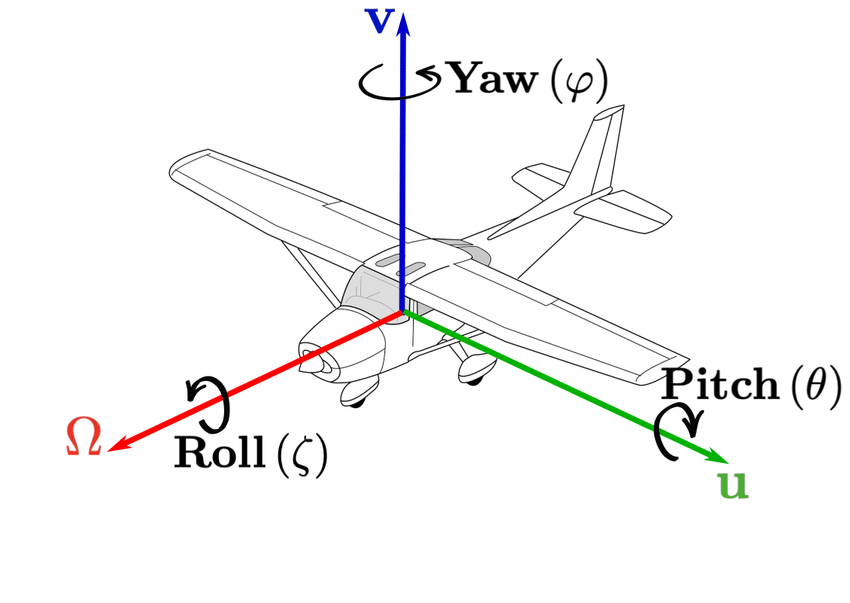
\includegraphics[width=0.5\textwidth]{pictures/pitch-roll-yaw.png.png}
        \caption{Example of drone orientation detection, showing the conversion of rotation vector (\texttt{rvec}) into Euler angles (Pitch, Roll, Yaw) \cite{researchgate_orientation}.}
        \label{fig:drone_orientation}
    \end{figure}

    \item \textbf{Yaw Validation:} The yaw angle (\texttt{yaw}) was particularly important to ensure the drone was correctly oriented to align with the charging station connectors. This orientation was visually validated on the interface, where the system displayed whether the drone's yaw was in the correct or incorrect orientation.
    \item \textbf{Detection Accuracy:} The markers were consistently detected under varying lighting conditions and angles, ensuring reliable data capture.
\end{itemize}

The system demonstrated robustness, maintaining consistent performance even when the markers were partially occluded or when the drone approached the markers at steep angles. This capability highlights the reliability of the system in real-world scenarios.

Additionally, the position and orientation data were published to a dedicated ROS 2 topic (\texttt{/aruco\_detection/compressed}), which allowed real-time visualization and logging of detection results for further analysis. The interface further utilized this data to provide visual feedback to the operator about the drone's yaw orientation. This feedback was critical for ensuring proper alignment with the charging station, as misalignment in yaw could prevent a secure connection.

\begin{figure}[H]
    \centering
    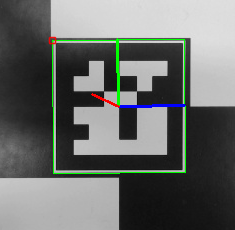
\includegraphics[width=0.4\textwidth]{pictures/aruco_detection.png}
    \caption{Real-time detection of ArUco markers, showing orientation and position axes.}
    \label{fig:aruco_detection_results}
\end{figure}

\subsection{Limitations and Observations}
\begin{itemize}
    \item The system's accuracy was dependent on the camera's calibration parameters. A well-calibrated camera ensured minimal distortion and higher precision in position and orientation calculations.
    \item Detection performance decreased slightly when the markers were too small or the drone was at a distance greater than 3 meters, emphasizing the importance of marker size and placement.
    \item While the system provided robust position and orientation data, it did not integrate an autonomous feedback loop to adjust the drone's position or orientation, as this was beyond the scope of this phase.
    \item The yaw validation feature was helpful for manual adjustments, but its effectiveness could be enhanced with automation in future iterations.
\end{itemize}

These results indicate that the vision system provides a solid foundation for potential future implementations involving autonomous navigation, precise landing, and improved yaw alignment for secure connections.

\section{Communication System}

The communication system was evaluated to ensure seamless interaction between the drone, the charging station, and the ground computer. The validation process focused on verifying that data exchange occurred reliably through WiFi using the ROS 2 framework.

\subsection{Validation of Communication System}

The communication system was verified through practical tests, ensuring that each component published and subscribed to the required topics as expected. The following steps summarize the validation process:

\begin{enumerate}
    \item \textbf{ROS 2 Topic Verification:}
    Using the command \texttt{ros2 topic list}, the list of active topics was inspected to confirm that the expected topics were available, including:
    \begin{itemize}
        \item \texttt{/camera\_image/compressed}: Published by the drone's companion computer.
        \item \texttt{/aruco\_detection/compressed}: Published by the ground computer after processing images.
        \item \texttt{/charging\_station/commands}: Commands sent from the ground computer to the charging station.
    \end{itemize}
    
    \item \textbf{Message Flow Test:}
    Each topic's message flow was monitored using the command:
    \begin{verbatim}
    ros2 topic echo <topic_name>
    \end{verbatim}
    For example:
    \begin{itemize}
        \item Confirming that the drone published images to \texttt{/camera\_image/compressed}.
        \item Verifying that the charging station responded to commands sent on \texttt{/charging\_station/commands}.
    \end{itemize}

    \item \textbf{End-to-End Test:}
    A complete end-to-end communication test was conducted:
    \begin{itemize}
        \item The drone published camera images to the ground computer.
        \item The ground computer processed these images and detected ArUco markers, publishing results to a new topic.
        \item Commands were sent to the charging station to open or close the drawer, completing the interaction loop.
    \end{itemize}
\end{enumerate}

\subsection{Results of Communication Validation}

The communication system functioned reliably under the following conditions:
\begin{itemize}
    \item \textbf{WiFi-Based Network:} Communication was stable within a local WiFi network, as no external Internet connection was required.
    \item \textbf{ROS 2 Middleware:} ROS 2 successfully handled the distributed communication, with nodes operating concurrently without delays.
    \item \textbf{Seamless Integration:} All devices (drone, charging station, and ground computer) interacted as intended, supporting the system's operational requirements.
\end{itemize}

This validation process demonstrated that the communication system met the design requirements, ensuring robust data exchange for monitoring and control.

\begin{figure}[H]
    \centering
    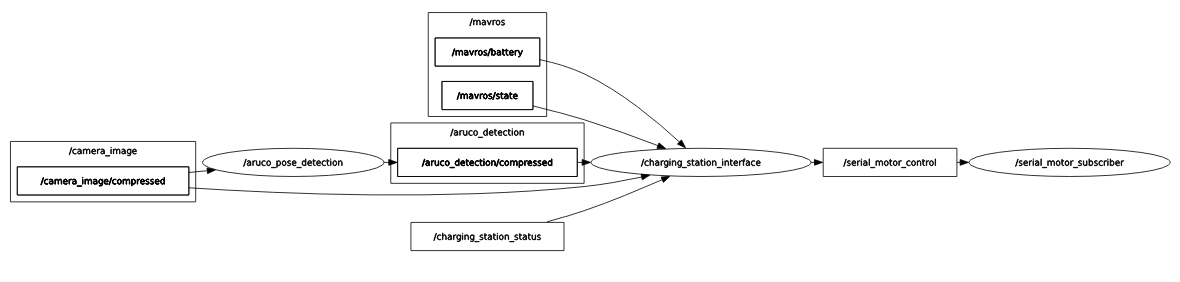
\includegraphics[width=1\textwidth]{pictures/complete_node_diagram.png}
    \caption{Diagram showcasing the communication architecture between the drone, charging station, and ground computer using ROS 2.}
    \label{fig:communication_validation}
\end{figure}

\section{General Performance Analysis}

\subsection{Global Integration Results}

The performance of the system was analyzed based on key metrics, comparing expected outcomes with actual observations:

\begin{itemize}
    \item \textbf{Drawer Operation:} The drawer mechanism operated smoothly and reliably during all tests, meeting the expected performance.
    \item \textbf{Battery Management:} While the charger slowed the battery discharge as expected, it did not provide significant charging capacity due to its limited power. This remains an area for improvement.
    \item \textbf{Communication Stability:} Data exchange between the drone, charging station, and ground computer was stable and reliable, fulfilling the expected requirements.
    \item \textbf{ArUco Detection Accuracy:} The system successfully detected the position and orientation of the drone relative to the ArUco markers, providing consistent and accurate results for real-time operations.
    \item \textbf{Drone Flight:} Manual flight was stable, and GPS-aided outdoor position control was achieved. However, indoor position-controlled flights were not conducted due to the lack of indoor positioning sensors.
\end{itemize}



